%%%%%%%%%%%%
%
% $Autor: Wings $
% $Datum: 2019-03-05 08:03:15Z $
% $Pfad: TemplateSensor $
% $Version: 4250 $
% !TeX spellcheck = en_GB/de_DE
% !TeX encoding = utf8
% !TeX root = filename 
% !TeX TXS-program:bibliography = txs:///biber
%
%%%%%%%%%%%%

\chapter{Anwendungsdatenformat}
	Dieses Kapitel beschreibt die Struktur der Anwendungsdaten, die innerhalb der beschriebenen Infrastruktur zur Kommunikation verwendet werden, sowie die Datenformate, die zur Konfiguration des Systems dienen. Zunächst werden die relevanten Datenformate anhand ausgewählter Beispiele erläutert.


\section{Sensorprofile \label{SA:SensorProfile}}
	
	Sensorprofile definieren die logische und binäre Abbildung einzelner Sensorwerte innerhalb des übertragenen \acs{lora}-Payloads. Sie beschreiben eindeutig, wie ein bestimmter Sensortyp in das Nutzdatenfeld kodiert wird, und bilden damit die zentrale Schnittstelle zwischen der Sensordatenerfassung auf dem Endgerät, der Payload-Erstellung sowie der serverseitigen Dekodierung.
	
	Da unterschiedliche Sensoren verschiedene Wertebereiche, Auflösungen und physikalische Grö{\ss}en besitzen, ist eine einheitliche Kodierung nicht praktikabel. Ein Sensorprofil legt daher für jeden unterstützten Sensortyp fest, wie der jeweilige Messwert vor der Übertragung skaliert, serialisiert und im Payload eindeutig identifiziert wird. Ohne diese Profile wäre eine korrekte Interpretation der kompakten und bandbreitenoptimierten \ac{lorawan}-Nutzdaten auf Serverseite nicht möglich.
	
	Ein Sensorprofil wird durch die Struktur \PYTHON{SensorProfile} beschrieben und besteht aus den folgenden Parametern:
	
	\begin{itemize}
		\item \PYTHON{SensorType} – Logischer Sensortyp zur eindeutigen Identifikation der Messgrö{\ss}e innerhalb der Firmware und auf Serverseite. Jeder Sensortyp referenziert genau einen physikalischen Sensor oder eine Messgrö{\ss}e und muss konsistent in der gesamten Systemkonfiguration verwendet werden.
		
		\item \PYTHON{profileNr} – Numerische Profilkennung, die im Payload übertragen wird und zur Identifikation des Sensorprofils bei der Dekodierung dient. Die vergebenen Profilnummern müssen eindeutig sein und dürfen sich innerhalb des Systems nicht wiederholen.
		
		\item \PYTHON{byteSize} – Anzahl der Bytes, die zur Kodierung des skalierten Sensorwerts im Payload verwendet werden. Dieser Parameter bestimmt unmittelbar die Länge des Payloads und ermöglicht eine präzise Abschätzung der maximalen Nutzdatenlänge.
		
		\item \PYTHON{scale} – Skalierungsfaktor, der vor der Serialisierung auf den gemessenen Flie{\ss}kommawert angewendet wird. Durch die Skalierung können physikalische Messwerte effizient als Ganzzahlen übertragen werden, ohne relevante Auflösung zu verlieren (siehe~\autoref{data:deviceProfileConfig}).
		
		\item \PYTHON{signedValue} – Kennzeichnung, ob der kodierte Messwert als vorzeichenbehafteter oder vorzeichenloser Integer interpretiert wird. Dadurch können sowohl positive als auch negative Messgrö{\ss}en abgebildet werden.
	\end{itemize}
	
	Die Sensorprofile werden zentral in der Firmware definiert und stehen allen Geräten, die diese Firmware verwenden, in identischer Form zur Verfügung. Die Gesamtheit der Profile wird in einer statischen Profiltabelle verwaltet und dient als Grundlage für die Payload-Erstellung, die Grö{\ss}enabschätzung der Nutzdaten sowie die Validierung gegen die maximal zulässige Payload-Länge.
	
	\autoref{code:sensorprofiles} zeigt die Implementierung der Sensorprofile in der Konfigurationsdatei \PYTHON{SensorProfiles.cpp}.
	{
		\captionof{code}{Konfigurationsdatei \PYTHON{SensorProfiles.cpp}}
		\label{code:sensorprofiles}
		\ArduinoExternal{}{../../Code/MKRWAN1310/SoftwareArchitecture/SensorProfiles.cpp}
	}
	
\paragraph{Auswahl von Bytelänge und Skalierungsfaktor \label{data:deviceProfileConfig}}
	Die Bytelänge bestimmt ausschlie{\ss}lich, wie viele Bytes ein Messwert im Payload belegt, und beeinflusst damit direkt die Payload-Grö{\ss}e. Der Skalierungsfaktor bestimmt hingegen die numerische Auflösung des Messwertes, indem er die Anzahl der dargestellten Nachkommastellen festlegt. Der Skalierungsfaktor hat keinen direkten Einfluss auf die Payload-Länge, kann jedoch eine grö{\ss}ere Bytelänge erforderlich machen, falls der skalierte Messwert den darstellbaren Integerbereich überschreitet.

\subparagraph{Beispielhafte Festlegung von Bytelänge und Skalierungsfaktor}

	Zur Verdeutlichung der Auswahl von Bytelänge und Skalierungsfaktor wird ein exemplarischer Lichtsensor betrachtet. Der Sensor liefert Messwerte im Bereich von $0$ bis $10\,000$. Die Sensorwerte liegen innerhalb der Firmware als Flie{\ss}kommazahlen vor und sollen im Payload als Ganzzahlen übertragen werden.
	
	Zunächst wird die gewünschte Auflösung festgelegt. Soll der Messwert ohne Nachkommastellen übertragen werden, wird ein Skalierungsfaktor von $s = 1$ gewählt. Der maximal zu kodierende Ganzzahlwert beträgt in diesem Fall
	\[
	10\,000 \cdot 1 = 10\,000.
	\]
	
	Ein vorzeichenloser Integer mit einer Bytelänge von $2$~Bytes kann Werte bis $65\,535$ darstellen, sodass der skalierte Messwert vollständig abgedeckt wird. Die Wahl von $2$~Bytes ist damit ausreichend und führt zu einer kompakten Payload-Darstellung.
	
	Soll hingegen eine höhere Auflösung erreicht werden, beispielsweise eine Nachkommastelle, wird der Skalierungsfaktor auf $s = 10$ erhöht. Der maximal zu kodierende Wert beträgt dann
	\[
	10\,000 \cdot 10 = 100\,000.
	\]
	
	Dieser Wert überschreitet den darstellbaren Bereich von $2$~Bytes und erfordert eine Bytelänge von $3$~Bytes. Durch die Erhöhung des Skalierungsfaktors verbessert sich die Auflösung des Messwertes, gleichzeitig steigt jedoch der Speicherbedarf im Payload.
	
	Dieses Beispiel zeigt, dass der Skalierungsfaktor die Auflösung bestimmt, während die Bytelänge den maximal darstellbaren Wertebereich begrenzt. Die Parameter sind daher stets gemeinsam zu betrachten und so zu wählen, dass eine ausreichende Auflösung bei minimaler Payload-Grö{\ss}e erreicht wird.

	
%	 Zusätzlich werden die Profildefinitionen während der Kompilation automatisch in einer JSON-Datei (\PYTHON{device\_profiles.json}) gespeichert, sodass diese auf den Server übertragen werden können. Auf diese Weise verfügen sowohl das Endgerät als auch der Server über denselben Satz von Profilen. Das Beispiel in \ref{code:sensorprofiles} zeigt die Struktur einer solchen JSON-Datei.
%	 
%		
%	
%	\begin{figure}[H]
%		\captionof{code}{Beispiel einer \PYTHON{device\_profiles.json}-Datei}
%%		\label{code:sensorprofiles}
%		\begin{verbatim}
%			[
%			{
%				"type": "CURRENT_SENSOR",
%				"profileNr": "1",
%				"bitSize": 4
%			},
%			{
%				"type": "TEMPERATURE_SENSOR",
%				"profileNr": "2",
%				"bitSize": 2
%			}
%			]
%		\end{verbatim}
%	\end{figure}
%	
%	\PYTHON{device\_profiles.json}-Datei listet alle Sensorprofile auf, die das Endgerät unterstützt. Damit die Anwendung die eingehenden Bytes korrekt dekodieren kann, muss dieselbe Profilliste ebenfalls im da vorhanden sein. Beim Hinzufügen eines neuen Sensors wird die JSON-Datei auf dem Endgerät automatisch aktualisiert. Anschlie{\ss}end muss sie mit der Datei auf der Anwendung abgeglichen werden, um sicherzustellen, dass beide Seiten über identische Profile verfügen. Wird ein neues, der Anwendung bislang unbekanntes Profil erzeugt, muss die entsprechende Datei auf der Anwendung um dieses Profil ergänzt werden.
%	

	
\section{Uplink-Payload}
	Die vom Nutzer übertragenen Anwendungsdaten werden im Feld \PYTHON{FRMPayload} des \acs{lorawan}-Payloads abgelegt (siehe~\autoref{lorawan:frmpayload}) . Im folgenden Kapitel bezieht sich der Begriff \PYTHON{Payload} daher ausschlie{\ss}lich auf das Feld \PYTHON{FRMPayload}, da die übrigen Bestandteile des \PYTHON{PHY-Payloads} zum MAC-Layer gehören und für den Benutzer nicht zugänglich sind.

	\medskip

	Jeder Endnode kann mit mehreren Sensoren ausgestattet werden. Aufgrund der \ac{lorawan}-Beschränkungen ist die Anzahl der übertragbaren Sensordaten jedoch limitiert. Die maximale Grö{\ss}e des Payloads (\PYTHON{FRMPayload}) beträgt bei der Datenrate~\PYTHON{DR0} 51~Bytes (als \PYTHON{MAX\_PAYLOAD\_BYTES} definiert) und bildet in dieser Anwendung die Obergrenze für die Menge an übertragbaren Sensordaten (siehe~\autoref{tab:lorawan-payload-m}, \autoref{openPoints:LoRaWANArch}). Davon werden 4~Bytes für standardisierte Metadaten reserviert (\PYTHON{Statusbytes}, \PYTHON{Akkulevel}, \PYTHON{ErrorCode} und \PYTHON{SensorsCnt}). Der verbleibende Speicherplatz steht für die \PYTHON{ProfileNr}-Bytes und Sensormesswerte zur Verfügung. Die resultierende \PYTHON{Payload} -Länge liegt somit zwischen 4~Bytes (nur Metadaten) und 51~Bytes - abhängig von Anzahl und Typ der angeschlossenen Sensoren.
	



\subsection{Struktur des Payloads}
Der \PYTHON{Payload}  wird für jedes Endgerät zur Laufzeit dynamisch erzeugt. Seine Struktur besteht unabhängig von der Anzahl der Sensoren grundsätzlich aus zwei logischen Bereichen:

\begin{itemize}
	\item \textbf{Header} - enthält:
		\begin{itemize}
			\item \PYTHON{Statusbytes}
			\item \PYTHON{Akkulevel}
			\item \PYTHON{ErrorCode}
			\item \PYTHON{SensorsCnt}
		\end{itemize}
	
	\item \textbf{Nutzdatenbereich} - enthalten Sensorprofile (\PYTHON{ProfileNr} - Bytes) und eigentliche Sensordaten entsprechend den im Header angegebenen Sensortypen.
\end{itemize}


	\begin{figure}[H]
		\centering
		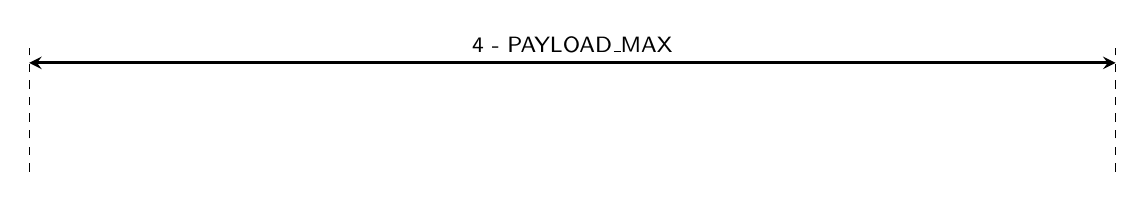
\begin{tikzpicture}[scale=0.92]
			\tikzset{
				node distance=0.5cm and 0.4cm,
				textDef/.style={font=\sffamily\footnotesize,},
				lineDef/.style={line width={2pt}},
				arrowStyle/.style={line width=1pt, >=stealth, black},
				boxDef/.style={
					draw,
					rectangle,
					rounded corners=1pt,
					minimum width=2.5cm,
					minimum height=0.7cm,
					align=center,
					fill=gray!20
				},
			}
			\SensorFRMPayloadDescription
			
			\draw[arrowStyle, <->, black] (0, 2.5) -- (15, 2.5) node[textDef, above, midway] {4 - \PYTHON{PAYLOAD\_MAX}};
			
			\foreach \x in {0, 15} {
				\draw[dashed] (\x, 1) -- (\x, 2.7);
			}
		\end{tikzpicture}
		\caption{Struktur des Payloads}
	\end{figure}

	
	\begin{table}[H]
		\caption{Beschreibung der einzelnen Bytes des Payload-Headers}
		\begin{tabularx}{\textwidth}{c|c|c|X|c}
			\hline
			\textbf{Name} & \textbf{Bytes} & \textbf{Typ} & \textbf{Beschreibung} & \textbf{Wertebereich} \\
			\hline
			
			Statusbyte & 1 & uint8\_t &
			Statusinformationen des Endgeräts (siehe Abschnitt~\ref{SA:PHYPayloadStatusBytes}). &
			0--255 \\
			\hline
			
			Akkustatus & 1 & uint8\_t &
			Ladestand der Batterie zum Zeitpunkt der Übertragung in Prozent. &
			0--100 \\
			\hline
			
			ErrorCode & 1 & uint8\_t &
			Fehlercode, der den aktuellen Fehlerzustand des Endgeräts beschreibt
			(siehe Abschnitt~\ref{SA:ErrorCodes}). &
			0--5 \\
			\hline
			
			SensorsCnt & 1 & uint8\_t &
			Anzahl der Sensoren, für die im Payload Messwerte übertragen werden. &
			0--255 \\
			\hline
			
			\PYTHON{profileNr} & 1 & uint8\_t &
			Profilkennung des Sensors, dessen Messwert im Anschluss übertragen wird
			(siehe Abschnitt~\ref{SA:SensorInfo}). &
			0--255 \\
			\hline
			
			Messwerte & variabel & -- &
			Sequenz der übertragenen Messwerte. Die Anzahl der Bytes pro Messwert
			wird durch das jeweilige Sensorprofil bestimmt
			(siehe Abschnitt~\ref{SA:SensorInfo}). &
			-- \\
			\hline
			
		\end{tabularx}
	\end{table}
	

	Sollte ein Endgerät keine Sensoren enthalten, werden keine \PYTHON{profileNr}-Bytes in den Header geschrieben. In diesem Fall besteht der Payload ausschlie{\ss}lich aus den standardisierten Metadaten ohne Messwertdaten.
	

\subsection{Struktur der Statusbytes \label{SA:PHYPayloadStatusBytes}}
\begin{center}
	\begin{tikzpicture}
		\ParamBytePayload
	\end{tikzpicture}
	\captionof{figure}{Bitstruktur von Byte \PYTHON{Statusbyte}}
\end{center}

\begin{table}[H]
	\caption{Bitweise Beschreibung von \PYTHON{Statusbyte}}
	\begin{tabularx}{\textwidth}{c|X|X}
		\hline
		\textbf{Bit} & \textbf{Funktion} & \textbf{Bedeutung} \\
		\hline
		0 & Spannungsversorgung 
		& 1 - Externe Spannungsversorgung vorhanden \newline
		0 - Akkubetrieb \\
		\hline
		1 & Neustartindikator 
		& 1 - Gerät wurde seit dem letzten Uplink neu gestartet \newline
		0 - Kein Neustart seit dem letzten Uplink \\
		\hline
		2 & Fehlerstatus 
		& 1 - Fehlerzustand aktiv (Sensorfehler oder interne Fehlfunktion) \newline
		0 - Kein Fehler vorhanden \\
		\hline
		3--7 & (Derzeit nicht verwendet) & Reserviert für zukünftige Erweiterungen \\
		\hline
	\end{tabularx}
\end{table}

\subsection{Struktur der ErrorCodes \label{SA:ErrorCodes}}
	Die ErrorCodes werden vom Endgerät gesetzt, sobald während des Betriebs ein Fehler auftritt. Sie ermöglichen der Anwendung eine eindeutige Klassifikation des Fehlerzustands sowie eine gezielte Reaktion auf unterschiedliche Fehlerszenarien.
	\begin{table}[H]
		\caption{Übersicht der ErrorCodes}
		\begin{tabularx}{\textwidth}{c|c|X}
			\hline
			\textbf{Name} & \textbf{Code} & \textbf{Beschreibung} \\
			\hline
			
			NONE & 0 &
			Kein Fehler vorhanden. Das Endgerät arbeitet fehlerfrei. \\
			\hline
			
			NO\_SENSORS\_ACTIVE & 1 &
			Es sind keine Sensoren aktiv oder initialisiert. \\
			\hline
			
			NO\_VALID\_SENSOR\_DATA & 3 &
			Es wurden keine gültigen Messwerte von den aktiven Sensoren erfasst. \\
			\hline
			
			PAYLOAD\_BUILD\_FAILED & 4 &
			Der Payload konnte aufgrund eines internen Fehlers nicht erstellt werden. \\
			\hline
			
			PAYLOAD\_TOO\_LARGE & 5 &
			Die erzeugten Nutzdaten überschreiten die maximal zulässige Payload-Grö{\ss}e. \\
			\hline
			
		\end{tabularx}
	\end{table}
	


\section{\PYTHON{ProfilNr} und Messwerte im \PYTHON{Payload}  \label{SA:SensorInfo}}

Die Bytes der Felder \PYTHON{ProfilNr} und \textit{Messwerte} stehen in einem direkten Zusammenhang. 
Die \PYTHON{ProfilNr}-Bytes definieren die Sensorprofile (siehe~\ref{SA:SensorProfile}), die angeben um welchen Sensortyp es sich handelt, und geben gleichzeitig an, wie viele Bytes im \PYTHON{Payload}  für den jeweiligen Messwert vorgesehen sind. Damit der \PYTHON{Payload}  korrekt kodiert bzw. dekodiert werden kann, müssen der Endnode und die Anwendung dieselben Sensorprofile kennen. Der Endnode erstellt den \PYTHON{Payload}  anhand der konfigurierten Profile, während die Anwendung diesen anhand derselben Profile dekodiert.

\subsection{\PYTHON{ProfilNr}-Bytes}
	
	Die \PYTHON{ProfilNr}-Bytes befinden sich im Header ab Position~5 Jedes Profil (in der \autoref{fig:AW:ProfilBytesEx} \PYTHON{\(X_1\)}, \PYTHON{\(X_2\)}) wird durch genau \textbf{ein Byte} (\PYTHON{uint8\_t}) repräsentiert. Es können beliebig viele Profile angegeben werden, solange die Gesamtlänge des Payloads den Wert \PYTHON{MAX\_PAYLOAD\_BYTES} nicht überschreitet. Dabei muss beachtet werden, dass \textbf{für jedes \PYTHON{ProfilNr}-Byte} auch ein entsprechender Messwert übertragen wird (siehe~\ref{LoRaWANArch:Values}).
	
	\begin{figure}[H]
		\centering
		
\begin{tikzpicture}[scale=0.92]
			\tikzset{
				node distance=0.5cm and 0.4cm,
				textDef/.style={font=\sffamily\small,},
				lineDef/.style={line width={2pt}},
				arrowStyle/.style={line width=2pt, >=stealth, red},
			}
			\SensorFRMPayload
			
			\fill[gray, opacity=0.5] (0, 0) rectangle (4, 1);
			\fill[gray, opacity=0.5] (7, 0) rectangle (15, 1);
			\draw[line width=1.5pt, dashed] (3.8, -0.2) rectangle (7.2, 1.2);
			
			\draw[arrowStyle, <-] (4.25, -0.1) -- ++(-0.25, -0.5) node[textDef,below] {\shortstack{\PYTHON{ProfilNr} 1}};
			\draw[arrowStyle, <-] (5.5, -0.1) -- ++(0, -1) node[textDef,below] {\shortstack{\PYTHON{ProfilNr} 2}};
			\draw[arrowStyle, <-] (6.75, -0.1) -- ++(0.25, -0.5) node[textDef,below] {\shortstack{\PYTHON{ProfilNr} n}};
		\end{tikzpicture}
		\caption{Position der \PYTHON{ProfilNr}-Bytes im \PYTHON{Payload} }
		\label{fig:AW:ProfilBytesEx}
	\end{figure}

\subsection{Messwerte \label{LoRaWANArch:Values}}

	Die Messwerte werden als eine Reihe von Bytes (\PYTHON{uint8\_t}) übertragen. Anzahl der Messwerte entspricht immer der Anzahl der verwendeten \PYTHON{ProfilNr}-Einträge. 
	Die Messwerte werden in derselben Reihenfolge in den Payload geschrieben, in der auch die Profile im Header angegeben wurden.

	\begin{figure}[H]
		\centering
		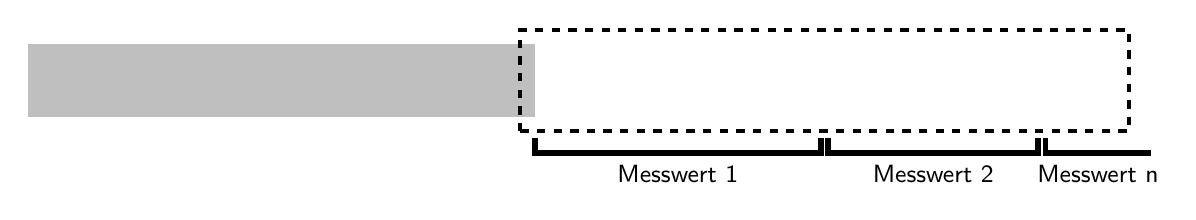
\begin{tikzpicture}[scale=0.92]
			\tikzset{
				node distance=0.5cm and 0.4cm,
				textDef/.style={font=\sffamily\small,},
				lineDef/.style={line width={2pt}},
				arrowStyle/.style={line width=2pt, >=stealth, red},
			}
			\SensorFRMPayload
			
			\fill[gray, opacity=0.5] (0, 0) rectangle (7, 1);
			\draw[line width=1.5pt, dashed] (6.8, -0.2) rectangle (15.2, 1.2);
			
			%\draw[arrowStyle, <-] (2.25, -0.1) -- ++(-0.25, -0.5) node[textDef,below] {\shortstack{\PYTHON{ProfileNr} 1}};
			%\draw[arrowStyle, <-] (3.5, -0.1) -- ++(0, -1) node[textDef,below] {\shortstack{\PYTHON{ProfileNr} 2}};
			%\draw[arrowStyle, <-] (4.75, -0.1) -- ++(0.25, -0.5) node[textDef,below] {\shortstack{\PYTHON{ProfileNr} n}};
			\draw[lineDef] (7, -0.3) -- ++(0, -0.2) -- (10.95, -0.5) node[textDef, midway, below] {\shortstack{\PYTHON{Messwert 1}}} -- (10.95, -0.3);
			\draw[lineDef] (11.05, -0.3) -- ++(0, -0.2) -- (13.95, -0.5) node[textDef, midway, below] {\shortstack{\PYTHON{Messwert 2}}} -- (13.95, -0.3);
			\draw[lineDef] (14.05, -0.3) -- ++(0, -0.2) -- (15.5, -0.5) node[textDef, midway, below] {\shortstack{\PYTHON{Messwert n}}};
			
		\end{tikzpicture}
		\captionof{figure}{Anordnung der Messwerte}
	\end{figure}
	
\subsubsection{Kodierung der Messwerte}

Die Kodierung der Messwerte erfolgt vollständig profilbasiert und unabhängig von den internen Datentypen der Firmware. Jeder Messwert wird vor der Übertragung gemä{\ss} den im zugehörigen Sensorprofil definierten Parametern skaliert und anschlie{\ss}end als ganzzahliger Wert in den \PYTHON{Payload} serialisiert.

Zunächst wird der erfasste Messwert, der intern als Flie{\ss}kommazahl (\PYTHON{float}) vorliegt, mit dem im Sensorprofil definierten Skalierungsfaktor multipliziert. Dadurch können physikalische Messgrö{\ss}en mit einer definierten Auflösung effizient als Ganzzahlen übertragen werden. Die resultierende skalierte Grö{\ss}e wird anschlie{\ss}end in einen ganzzahligen Wert konvertiert. Abhängig vom Profil wird der Wert dabei entweder als vorzeichenbehaftet oder vorzeichenlos interpretiert.

Die eigentliche Serialisierung erfolgt byteweise. Hierbei werden ausschlie{\ss}lich die im Sensorprofil definierte Anzahl der niederwertigsten Bytes (\PYTHON{byteSize}) des ganzzahligen Wertes in den \PYTHON{Payload} geschrieben. Die Kodierung erfolgt im Little-Endian-Format, sodass das niederwertigste Byte zuerst übertragen wird. Eine bitweise Packung einzelner Messwerte wird bewusst nicht eingesetzt, um die Dekodierung auf der Serverseite zu vereinfachen und die Rechenkomplexität im Endgerät gering zu halten.

Die Länge eines kodierten Messwertes ist somit nicht an einen konkreten C++-Datentyp gebunden, sondern wird ausschlie{\ss}lich durch das Sensorprofil bestimmt. Dadurch können unterschiedliche Auflösungen und Wertebereiche flexibel abgebildet werden, ohne die Payload-Struktur zu verändern.

\begin{figure}[H]
	\captionof{code}{Beispielhafte Kodierung eines skalierten Messwertes in den \PYTHON{Payload}}
	\begin{verbatim}
		// Skalierter Messwert
		int64_t v = (int64_t)(sensorValue * scale);
		
		// Unsigned-Werte werden auf 0 begrenzt
		if (!signedValue && v < 0)
		v = 0;
		
		// Schreiben der niederwertigsten Bytes (Little-Endian)
		for (uint8_t i = 0; i < byteSize; ++i) {
			payload[offset + i] = (v >> (8 * i)) & 0xFF;
		}
	\end{verbatim}
\end{figure}

	%Da der Arduino Little-Endian verwendet, erscheinen die Bytes des Messwertes im Payload ebenfalls in Little-Endian-Reihenfolge. Für die korrekte Dekodierung muss der Server daher aus dem Sensorprofil sowohl die Byteanzahl als auch den zugrunde liegenden Datentyp kennen, um den Messwert aus den Rohbytes  rekonstruieren zu können.


\subsection{Beispiel für die Belegung der \PYTHON{ProfileNr}- Bytes und der Messwerte}
	Angenommen, es stehen folgende vordefinierte Profile zur Verfügung:

\begin{figure}[H]
	\captionof{code}{Beispiel einer \PYTHON{device\_profiles.json}-Datei}
	\begin{verbatim}
		{
			"1": {
				"type": "CURRENT_SENSOR",
				"profileNr": 1,
				"byteSize": 4,
				"scale": 1000,
				"signedValue": true
			},
			"2": {
				"type": "TEMPERATURE_SENSOR",
				"profileNr": 2,
				"byteSize": 2,
				"scale": 100,
				"signedValue": true
			},
			"3": {
				"type": "SWITCH_SENSOR",
				"profileNr": 3,
				"byteSize": 1,
				"scale": 1,
				"signedValue": false
			}
		}
	\end{verbatim}
\end{figure}

	
	
	\begin{table}[H]
		\centering
		\caption{Definierte Sensortypen}
		\begin{tabular}{c|c|c|c}
			\hline
			Sensor & Profil & \PYTHON{ProfileNr} (HEX) & byteSize\\
			\hline
			Stromsensor & \PYTHON{CURRENT\_SENSOR} & \PYTHON{1} (0x01) & 4  \\
			\hline
			Temperatursensor & \PYTHON{TEMPERATURE\_SENSOR} & \PYTHON{2} (0x02) & 2 \\
			\hline
			Switch & \PYTHON{SWITCH\_SENSOR} & \PYTHON{3} (0x03) & 1 \\
			\hline
		\end{tabular}
	\end{table}
	
\subsubsection{Beispiel 1}

	Für die folgende Reihenfolge der Sensorprofile:
	\begin{enumerate}
		\item Stromsensor
		\item Temperatursensor
		\item Switch
	\end{enumerate}
	
	ergibt sich die entsprechende Belegung der Messwertbytes im Payload:
	
	
	\begin{figure}[H]
		\centering
		\begin{tikzpicture}[scale=0.92]
			\tikzset{
				node distance=0.5cm and 0.4cm,
				textDef/.style={font=\sffamily\footnotesize, red},
				lineDef/.style={line width={2pt}},
				arrowStyle/.style={line width=1pt, >=stealth, red},
				boxDef/.style={
					draw,
					rectangle,
					rounded corners=1pt,
					minimum width=2.5cm,
					minimum height=0.7cm,
					align=center,
					fill=gray!20
				},
			}
			
			\draw[black, thick] (-1,0) rectangle (2,1);
			\draw[black, thick] (2,0) rectangle (5,1);
			\draw[black, thick] (5,0) rectangle (6,1);
			\draw[black, thick] (5,0) rectangle (13,1);
			
			\foreach \x in {0, ..., 3}{
				\draw[black] (\x, 0) -- (\x, 1);
				\pgfmathsetmacro{\i}{int(\x + 1)}
				\node at (\x-0.5, 0.5) {\i};
			}
			
			\foreach \x in {3, 4}{
				\draw[black] (\x, 0) -- (\x, 1);
				\pgfmathsetmacro{\i}{int(\x - 2)}
				%\node at (\x-0.5, 0.5) {\(X_{\i}\)};
			}
			
			\foreach \x in {7, ..., 10}{
				\draw[black] ({\x}, 0) -- ({\x}, 1);
				\pgfmathsetmacro{\i}{int(\x - 6)}
				\node at (\x-0.5, 0.5) {\(Y_{1\i}\)};
			}
			
			\foreach \x in {11, ..., 12}{
				\draw[black] ({\x}, 0) -- ({\x}, 1);
				\pgfmathsetmacro{\i}{int(\x - 10)}
				\node at (\x-0.5, 0.5) {\(Y_{2\i}\)};
			}
			
			\node at (12.5, 0.5) {\(Y_{31}\)};
			
			% Sensor Profiles
			\node at (3.5, 0.5) {\PYTHON{0x01}};
			\node at (4.5, 0.5) {\PYTHON{0x02}};
			\node at (5.5, 0.5) {\PYTHON{0x03}};
			
			% Group Bytes
			\fill[green, thick,  fill opacity=0.2] (-1,0) rectangle ++(1,1);
			\fill[yellow, thick,  fill opacity=0.2] (-0,0) rectangle ++(1,1);
			\fill[Cyann, thick,  fill opacity=0.2] (1,0) rectangle ++(1,1);
			\fill[red, thick,  fill opacity=0.2] (2,0) rectangle ++(1,1);
			\fill[blue, thick,  fill opacity=0.2] (3,0) rectangle (6,1);
			\fill[gray, thick, fill opacity=0.2] (6,0) rectangle (13,1);
			
			\draw[lineDef] (6, -0.2) -- ++(0, -0.2) -- (9.95, -0.4) node[textDef, midway, below] {\shortstack{\PYTHON{Messwert 1}}} -- (9.95, -0.2);
			\draw[lineDef] (10.05, -0.2) -- ++(0, -0.2) -- (12, -0.4) node[textDef, midway, below] {\shortstack{\PYTHON{Messwert 2}}} -- (12, -0.2);
			\draw[lineDef] (12, 1.2) -- ++(0, 0.2) -- (13, 1.4) node[textDef, midway, above] {\shortstack{\PYTHON{Messwert 3}}} -- (13, 1.2);
			%\draw[arrowStyle, <-] (12.5, -0.2) -- ++(0, -0.5) node[textDef, below] {\PYTHON{Messwert 3}};
			
			\draw[arrowStyle, ->] (3.5, -0.2) -- ++(0, -1.0) -| (8, -0.8);
			\draw[arrowStyle, ->] (4.5, -0.2) -- ++(0, -1.3) -| (11, -0.8);
			\draw[arrowStyle, ->] (5.5, 1.2) -- ++(0, 1.0) -| (12.5, 1.8);
		\end{tikzpicture}
		\captionof{figure}{Belegung der Messwerte im Payload}
	\end{figure}

\subsubsection{Beispiel 2}
		Für die folgende Reihenfolge der Sensorprofile:
	\begin{enumerate}
		\item Temperatursensor
		\item Temperatursensor
		\item Switch
		\item Temperatursensor
	\end{enumerate}
	
	ergibt sich die entsprechende Belegung der Messwertbytes im Payload:
	
	\begin{figure}[H]
		\centering
		\begin{tikzpicture}[scale=0.9]
			\tikzset{
				node distance=0.5cm and 0.4cm,
				textDef/.style={font=\sffamily\footnotesize, red},
				lineDef/.style={line width={2pt}},
				arrowStyle/.style={line width=1pt, >=stealth, red},
				boxDef/.style={
					draw,
					rectangle,
					rounded corners=1pt,
					minimum width=2.5cm,
					minimum height=0.7cm,
					align=center,
					fill=gray!20
				},
			}
			
			\draw[black, thick] (-1,0) rectangle (2,1);
			\draw[black, thick] (2,0) rectangle (6,1);
			\draw[black, thick] (6,0) rectangle (7,1);
			\draw[black, thick] (5,0) rectangle (14,1);
			
			\foreach \x in {0, ..., 3}{
				\draw[black] (\x, 0) -- (\x, 1);
				\pgfmathsetmacro{\i}{int(\x + 1)}
				\node at (\x-0.5, 0.5) {\i};
			}
			
			\foreach \x in {3, 4}{
				\draw[black] (\x, 0) -- (\x, 1);
				\pgfmathsetmacro{\i}{int(\x - 2)}
				%\node at (\x-0.5, 0.5) {\(X_{\i}\)};
			}
			
			\foreach \x in {8, ..., 9}{
				\draw[black] ({\x}, 0) -- ({\x}, 1);
				\pgfmathsetmacro{\i}{int(\x - 6)}
				\node at (\x-0.5, 0.5) {\(Y_{1\i}\)};
			}
			
			\foreach \x in {10, ..., 11}{
				\draw[black] ({\x}, 0) -- ({\x}, 1);
				\pgfmathsetmacro{\i}{int(\x - 10)}
				\node at (\x-0.5, 0.5) {\(Y_{2\i}\)};
			}
			
			\node at (11.5, 0.5) {\(Y_{41}\)};
			
			\foreach \x in {13, ..., 14}{
				\draw[black] ({\x-1}, 0) -- ({\x-1}, 1);
				\pgfmathsetmacro{\i}{int(\x - 10)}
				\node at (\x-0.5, 0.5) {\(Y_{2\i}\)};
			}
			
			
			% Sensor Profiles
			\node at (3.5, 0.5) {\PYTHON{0x02}};
			\node at (4.5, 0.5) {\PYTHON{0x02}};
			\node at (5.5, 0.5) {\PYTHON{0x03}};
			\node at (6.5, 0.5) {\PYTHON{0x02}};
			
			% Group Bytes
			\fill[green, thick,  fill opacity=0.2] (-1,0) rectangle ++(1,1);
			\fill[yellow, thick,  fill opacity=0.2] (-0,0) rectangle ++(1,1);
			\fill[Cyann, thick,  fill opacity=0.2] (1,0) rectangle ++(1,1);
			\fill[red, thick,  fill opacity=0.2] (2,0) rectangle ++(1,1);
			\fill[blue, thick,  fill opacity=0.2] (3,0) rectangle (7,1);
			\fill[gray, thick, fill opacity=0.2] (7,0) rectangle (14,1);
			
			\draw[lineDef] (7, -0.2) -- ++(0, -0.2) -- (8.95, -0.4) node[textDef, midway, below] {\shortstack{\PYTHON{Messwert 1}}} -- (8.95, -0.2);
			\draw[lineDef] (9.05, -0.2) -- ++(0, -0.2) -- (11, -0.4) node[textDef, midway, below] {\shortstack{\PYTHON{Messwert 2}}} -- (11, -0.2);
			\draw[lineDef] (11, 1.2) -- ++(0, 0.2) -- (12, 1.4) node[textDef, midway, above] {\shortstack{\PYTHON{Messwert 3}}} -- (12, 1.2);
			\draw[lineDef] (12, -0.2) -- ++(0, -0.2) -- (14, -0.4) node[textDef, midway, below] {\shortstack{\PYTHON{Messwert 4}}} -- (14, -0.2);
			%\draw[arrowStyle, <-] (12.5, -0.2) -- ++(0, -0.5) node[textDef, below] {\PYTHON{Messwert 3}};
			
			\draw[arrowStyle, ->] (3.5, -0.2) -- ++(0, -1.0) -| (8, -0.8);
			\draw[arrowStyle, ->] (4.5, -0.2) -- ++(0, -1.3) -| (10, -0.8);
			\draw[arrowStyle, ->] (5.5, 1.2) -- ++(0, 1.0) -| (11.5, 1.8);
			\draw[arrowStyle, ->] (6.5, -0.2) -- ++(0, -1.6) -| (13, -0.8);
		\end{tikzpicture}
		\captionof{figure}{LoRaWAN Architektur}
	\end{figure}
	
	
	
%%%%%%%%%%%%%%%%%%%%%%%%%%%%%%%%%%%%%%%
\section{MQTT-Publikation \label{dataFormatt:mqtt}}

\begin{center}
	\begin{tikzpicture}
		\tikzset{
			node distance=0.5cm and 0.4cm,
			textDef/.style={font=\sffamily\small,},
			lineDef/.style={line width={2pt}},
			arrowStyle/.style={line width=2pt, >=stealth, red},
		}
		\serverNode{0.6}{0}{0}{0}{S1}
		\serverNode{0.6}{0}{7}{0}{A1}
		
		\draw[arrowStyle, ->] (S1.east) -- (A1.west) node[midway, above, textDef, text=black] {MQTT JSON Payload};
		
		\node[textDef, below= of S1.south] {\shortstack{LoRaWAN\\Server}};
		\node[textDef, below= of A1.south] {\shortstack{Anwendung}};
		
	\end{tikzpicture}
	\captionof{figure}{Kommunikationsfluss zwischen LoRaWAN-Server und Anwendung}
\end{center}
Die MQTT-Schnittstelle bildet die zentrale Kommunikationsschicht zwischen dem ChirpStack Application Server und der Backend-Applikation. Sie dient der Übertragung von Uplink-Nachrichten (Messwerte des Endgeräts). Die Kommunikation erfolgt über einen MQTT-Broker, der auf dem ChirpStack-Server bereitgestellt wird.

\subsubsection{Uplink-Themenstruktur}
Eingehende Messdaten des Endgeräts werden vom Application Server dekodiert und in strukturierter Form über folgende Topic-Hierarchie veröffentlicht:

\begin{verbatim}
	application/<application_id>/device/<dev_eui>/event/up
\end{verbatim}

Der Payload enthält ein JSON-Dokument, das sowohl die dekodierten Messwerte aus dem Uplink-PHY-Payload als auch Metadaten wie Zeitstempel, \PYTHON{DevEUI}, \PYTHON{RSSI} und \PYTHON{SNR} umfasst. Ein Beispiel für einen Uplink ist:

\begin{verbatim}
	{
		"deduplicationId":"2b85bbc4-a968-47a8-a25e-915ed16b36cd",
		"time":"2025-12-03T11:39:33.280681+00:00",
		"deviceInfo":{
			"tenantId":"15d825fb-60a7-4821-a014-691dc41a0758",
			"tenantName":"ChirpStack",
			"applicationId":"12f80a93-5419-4211-a990-24769dab576e",
			"applicationName":"MKRWAN1310",
			"deviceProfileId":"a75c5ec3-a8f0-44e3-805f-b8191d35bfdb",
			"deviceProfileName":"MKRWan1310",
			"deviceName":"TestDevice1",
			"devEui":"a8610a3539397f06",
			"deviceClassEnabled":"CLASS_A",
			"tags":{}
		},
		"devAddr":"005741ec",
		"adr":true,
		"dr":0,
		"fCnt":0,
		"fPort":2,
		"confirmed":false,
		"data":"MDExMjU3Q0RDQzVENDIwMDAwNTg0Mg==",
		"object":{
			"payload":"011257CDCC5D4200005842"
		},
		"rxInfo":[
		{"gatewayId":"5031395332214750",
			"uplinkId":17665,
			"gwTime":"2025-12-03T11:39:33.280681+00:00",
			"nsTime":"2025-12-03T11:39:35.928719679+00:00",
			"rssi":-89,"snr":-19.0,
			"channel":7,
			"location":{},
			"context":"W5xF9A==",
			"crcStatus":"CRC_OK"}
		],
		"txInfo":{
			"frequency":867900000,
			"modulation":{
				"lora":{
					"bandwidth":125000,
					"spreadingFactor":12,
					"codeRate":"CR_4_5"}
			}
		},
		"regionConfigId":"eu868"
	}
\end{verbatim}


	\medskip

	Der Payload besteht in diesem Beispiel aus insgesamt 11 Bytes: \PYTHON{011257CDCC5D4200005842}. 

	Die Anwendung extrahiert auf Grundlage der Sensorprofile (siehe~\ref{SA:SensorProfile}) die entsprechenden Felder, interpretiert die übertragenen Messwerte und speichert oder visualisiert diese anschlie{\ss}end. Die Zuordnung der Messdaten zu einem bestimmten Endgerät erfolgt über die in der JSON-Datei enthaltene \PYTHON{devEui}.




%	\subsubsection{Downlink-Themenstruktur}
%	Zum Versenden von Konfigurations- oder Steuerbefehlen stellt der Application Server ein dediziertes Downlink-Topic bereit:
%	
%	\begin{verbatim}
	%		application/<application_id>/device/<dev_eui>/command/down
	%	\end{verbatim}
%	
%	Downlinks werden in Form eines JSON-Dokuments publiziert, das den zu sendenden LoRaWAN-Payload (Base64-kodiert) sowie optionale Parameter wie FPort oder Wiederholungslogik enthält:
%	
%	\begin{verbatim}
	%		{
		%			"devEui": "a8610a3539397f06",
		%			"confirmed": true,
		%			"fPort": 10,
		%			"data": "MDI="
		%		}
	%		
	%	\end{verbatim}
%	
%	Der ChirpStack Application Server plant den Versand automatisch für das nächste verfügbare Empfangsfenster 
